\documentclass[border=2pt]{standalone}
\usepackage{tikz}
\usetikzlibrary{positioning, arrows.meta, calc}
\begin{document}
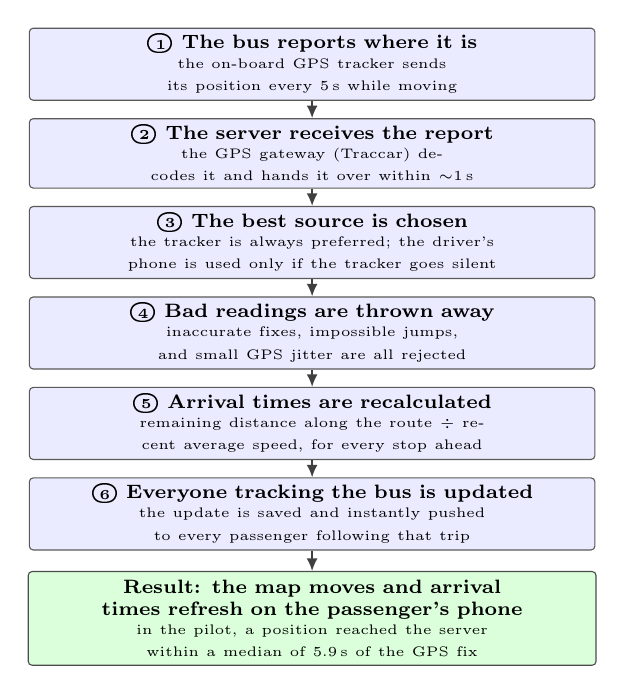
\begin{tikzpicture}[
  font=\scriptsize,
  stp/.style={draw=black!65, rounded corners=1.4pt, align=center, fill=blue!8,
               text width=70mm, inner sep=2.6pt},
  res/.style={draw=black!70, rounded corners=1.4pt, align=center, fill=green!14,
              text width=70mm, inner sep=3pt},
  sarr/.style={-{Latex[length=1.6mm,width=1.4mm]}, semithick, draw=black!75}
]
\newcommand{\stnum}[1]{\textbf{\textcircled{\raisebox{-0.4pt}{\tiny #1}}}}
\node[stp] (a)
  {\stnum{1} \textbf{The bus reports where it is}\\[-1pt]
   {\tiny the on-board GPS tracker sends its position every 5\,s while moving}};
\node[stp, below=2.2mm of a] (b)
  {\stnum{2} \textbf{The server receives the report}\\[-1pt]
   {\tiny the GPS gateway (Traccar) decodes it and hands it over within $\sim$1\,s}};
\node[stp, below=2.2mm of b] (c)
  {\stnum{3} \textbf{The best source is chosen}\\[-1pt]
   {\tiny the tracker is always preferred; the driver's phone is used only if the tracker goes silent}};
\node[stp, below=2.2mm of c] (d)
  {\stnum{4} \textbf{Bad readings are thrown away}\\[-1pt]
   {\tiny inaccurate fixes, impossible jumps, and small GPS jitter are all rejected}};
\node[stp, below=2.2mm of d] (e)
  {\stnum{5} \textbf{Arrival times are recalculated}\\[-1pt]
   {\tiny remaining distance along the route $\div$ recent average speed, for every stop ahead}};
\node[stp, below=2.2mm of e] (f)
  {\stnum{6} \textbf{Everyone tracking the bus is updated}\\[-1pt]
   {\tiny the update is saved and instantly pushed to every passenger following that trip}};
\node[res, below=2.6mm of f] (g)
  {\textbf{Result: the map moves and arrival times refresh on the passenger's phone}\\[-1pt]
   {\tiny in the pilot, a position reached the server within a median of 5.9\,s of the GPS fix}};
\foreach \x/\y in {a/b, b/c, c/d, d/e, e/f, f/g}{
  \draw[sarr] (\x.south) -- (\y.north);}
\end{tikzpicture}
\end{document}
